%!TEX root = ../DissertationDefensePresentation.tex

%%--------------------------------------------------------------------------------------------

\subsection*{Backup}

%%--------------------------------------------------------------------------------------------

\begin{frame}
	\begin{block}{}
		\begin{center}
			\shadowoffset{2pt}
			\shadowcolor{tamugold}
			\shadowtext{{\fontsize{30}{60}\selectfont \textbf{\textcolor{tamumaroon}{Backup Slides}}}}
			\vspace{1.5mm}
		\end{center}
	\end{block}
\end{frame}

\begin{frame}
	\frametitle{Datasets \& MC Samples}
	\label{frame:datasets_and_mc_samples}
	\vspace*{-0.24cm}
	\begin{block}{}
	\begin{itemize}
		\item Data:
		\begin{itemize}
			\item Using the full 2012 single electron (muon) datasets at \CM{8\tev} for 19.148\fbinv (19.279\fbinv)
		\end{itemize}
		\item MC Backgrounds:
		\begin{itemize}
			\item Dominant backgrounds (\Wjets, \ttbar, \Zjets) use Madgraph
			\item Diboson samples simulated using \textsc{pythia6}
			\item Single top samples simulated using \textsc{POWHEG}
		\end{itemize}
		\item Data-driven Backgrounds:
		\begin{itemize}
			\item The QCD sample is taken from data using an anti-isolation requirement
			%\item {\color{gray}W(l$\nu$)+Jets converted from a Z(ll)+Jets sample}
		\end{itemize}
		\item \HWW Samples:
		\begin{itemize}
			\item Generated using \textsc{POWHEG-BOX} and \textsc{pythia6}
			\item \tikzmark{signal1}{\ggH; $\MH=\text{125}\gev$; \HWWlvjj}
			\item \tikzmark{signal2}{\qqH; $\MH=\text{125}\gev$; \HWWlvjj}
			\item \tikzmark{signal3}{\WH, \ZH, \ttH; $\MH=\text{125}\gev$; \HWW}
		\end{itemize}
		\item Other Higgs Samples:
		\begin{itemize}
			\item \tikzmark{nsignal1}{\WH, \ZH, \ttH; $\MH=\text{125}\gev$; \HZZ}
			\item \tikzmark{nsignal2}{\ttH; \MH=125\gev; \Hbb }
			\item \tikzmark{nsignal3}{\WH; \MH=125\gev; \Hbb, $\W{\rightarrow}\Pl\cPgn$}
		\end{itemize}
	\end{itemize}
	\end{block}
	\tikz[overlay,remember picture]{\draw[draw=red,thick,fill opacity=0.2] ($(signal1)+(-0.5,0.3)$) rectangle ($(signal1)+(5.5,-0.1)$);}
	\tikz[overlay,remember picture]{\draw[draw=red,thick,fill opacity=0.2] ($(signal2)+(-0.5,0.3)$) rectangle ($(signal2)+(5.5,-0.1)$);}
	\tikz[overlay,remember picture]{\draw[draw=red,thick,fill opacity=0.2] ($(signal3)+(-0.5,0.3)$) rectangle ($(signal3)+(5.85,-0.1)$);}
	\tikz[overlay,remember picture]{\draw[draw=green,thick,fill opacity=0.2] ($(nsignal1)+(-0.5,0.3)$) rectangle ($(nsignal1)+(5.7,-0.1)$);}
	\tikz[overlay,remember picture]{\draw[draw=green,thick,fill opacity=0.2] ($(nsignal2)+(-0.5,0.3)$) rectangle ($(nsignal2)+(4.1,-0.1)$);}
	\tikz[overlay,remember picture]{\draw[draw=green,thick,fill opacity=0.2] ($(nsignal3)+(-0.5,0.3)$) rectangle ($(nsignal3)+(5.3,-0.1)$);}
\end{frame}

\begin{frame}<1>[label=frame:event_selection_signal_region]
	\frametitle{Event Selection}
	\vspace*{-0.24cm}
	\only<1>{%
		\begin{table}[tb]
			\centering
			\begin{tabular}{|l|c|c|}
			\hline
			\textbf{cut} & \textbf{electron channel} & \textbf{muon channel} \\
			\hline
			trigger type & single electron trigger & single muon trigger\\
			trigger name & HLT\_Ele27\_WP80\_v* & HLT\_{\color{red}Iso}Mu24\_eta2p1\_v* \\
			$E_{T}^{EE~\&~EB}\geqslant$ & 27\gev & - \\
			$ECalIso/E_{T}<$ & 0.15\text{ }(0.10) & - \\
			$HCalIso/E_{T}<$ & 0.10\text{ }(0.10) & - \\
			$TrkIso/E_{T}<$ & 0.05\text{ }(0.05) & - \\
			$p_{T}\geqslant$ & - & 24\GeV \\
			$|\eta|\leqslant$ & - & 2.1 \\
			$Isolation_{Relative}<$ & - & 0.15 \\ \hline
			\multicolumn{3}{|c|}{Lowest \textbf{un-prescaled} triggers} \\
			\multicolumn{3}{|c|}{Both triggers have some additional, more technical requirements} \\
			\hline
			\end{tabular}
		\end{table}
	}
	\only<2->{%
		\begin{table}[tb]
			\centering
			\begin{tabular}{|l|c|c|}
				\hline
				\textbf{cut} & \textbf{electron channel} & \textbf{muon channel} \\
				\hline
				trigger type & single electron trigger & single muon trigger\\
				vertex & $\geqslant1$ good primary vertex & $\geqslant1$ good primary vertex\\
				lepton $p_{T}>$ & $30\unit{GeV}$ & $25\unit{GeV}$\\
				lepton $|\eta|<$ & $2.5$ & 2.1\\
				lepton isolation & PF Isolation WP80 & PF Isolation $<0.12$\\
				jet $|\eta|<$ & 2.4 & 2.4\\
				leading jet $p_{T}>$ & $30\unit{GeV}$ & $30\unit{GeV}$\\
				all other jet $p_{T}>$ & $25\unit{GeV}$ & $25\unit{GeV}$\\
				$n_{b-jets}<$ & 1 & 1 \\
				Missing E\textsubscript{T}$>$ & $25\unit{GeV}$ & $25\unit{GeV}$\\ \hline
			\end{tabular}
		\end{table}
	}
	\vspace*{0.15cm}
	\onslide<2->{
	\begin{block}{}
		\begin{itemize}
			\item \textbf{Exactly 1 electron or muon} passing quality criteria
			\item \textbf{No additional loose leptons}
			\item \textbf{At least 2 Anti-k\textsubscript{T} PF$+$CHS, $R=0.5$} jets passing quality requirements
			\item b-jet veto used to remove a large portion of $t\bar{t}$ events
			\item Missing E\textsubscript{T} cut removes some of the QCD background
		\end{itemize}
	\end{block}
	}
\end{frame}
\againframe<2>{frame:event_selection_signal_region}

\begin{frame}
	\frametitle{Pileup Per ${\mu\times}A_{j}$}
	\vspace*{-0.24cm}
	\begin{center}
		\includegraphics[width=0.69\figwidth]{\figpath/offsetVsRcone_Eta00_pTOffset.pdf}
	\end{center}
\end{frame}

\begin{frame}
	\frametitle{Data-Driven QCD Model}
	\framesubtitle{$\eta$ Dependance}
	\vspace*{-0.60cm}
	\begin{center}
		\begin{aeq}{eq:N_QCD_sig}
			N_{antiIso}^{QCD}\left(\eta\right)s_{QCD}\left(\eta\right)=N_{signal\text{ }region}^{QCD}\left(\eta\right)
		\end{aeq}
		\includegraphics[width=0.76\textwidth]{\anpath/QCD_EtaWeights/AllMetFits_control6_electron.pdf}\\
		Very good fits!\\
		%\scriptsize{Note: See backup slides for the same plot in the $2+$ jets bin}
	\end{center}
	\begin{textblock}{0.30}(0.53,0.73)
		\begin{block}{}
			\textbf{\Huge{1 Jet Bin}}
		\end{block}
	\end{textblock}
\end{frame}

\frame{
	\frametitle{$\eta$ Corrections}
	\framesubtitle{$2+$ Jets (electron) Bin}
	\vspace*{-0.24cm}
	\begin{center}
		\includegraphics[width=0.8\textwidth]{/Users/aperloff/Documents/CMS/Notes_and_Papers/notes/AN-13-132/trunk/figures/QCD_EtaWeights/AllMetFits_signal_electron.pdf}
	\end{center}
}
\frame{
	\frametitle{$\eta$ Corrections}
	\framesubtitle{$2+$ Jets (muon) Bin}
	\vspace*{-0.24cm}
	\begin{center}
		\includegraphics[width=0.8\textwidth]{/Users/aperloff/Documents/CMS/Notes_and_Papers/notes/AN-13-132/trunk/figures/QCD_EtaWeights/AllMetFits_signal_muon.pdf}
	\end{center}
}

\begin{comment}
\begin{frame}
	\frametitle{Data-Driven QCD Model}
	\framesubtitle{$\eta$ Weights continued}
	\vspace*{-0.24cm}
	\begin{figure}
		\centering
		\begin{subfigure}[t]{0.49\textwidth}
			\includegraphics[width=\textwidth]{\figpath/LeptEta_2015_03_21_ValidationPlots_PU_CSV_TTbar_Jets2_electron.png}
		\end{subfigure}
		\hfill
		\begin{subfigure}[t]{0.49\textwidth}
			\includegraphics[width=\textwidth]{\figpath/LeptEta_2015_04_27_LimitHistograms_PU_CSV_TTbar_QCDEta_Scale_Jets2_electron.png}
		\end{subfigure}
	\end{figure}
	\begin{textblock}{0.30}(0.16,0.50){\Large\color{red}Pre-Correction}\end{textblock}
	\begin{textblock}{0.30}(0.65,0.50){\Large\color{red}Post-Correction}\end{textblock}
\end{frame}

\frame{
	\frametitle{QCD Sample Purity - Electron Channel}
	\vspace*{-0.24cm}
	\begin{columns}[T]
		\setlength{\residualSpace}{\textwidth-0.36\textwidth}%
		\column{0.33\textwidth}
			\vspace*{-0.24cm}
			\begin{block}{}
				\begin{itemize}
					\item These plots show the various regions of interest when analyzing the purity of the QCD sample
					\begin{itemize}
						\item Top Left: All events in data
						\item Top Right: Selected data
						\item Bottom Left: Selected QCD
						\item Bottom Right: All events in WJets MC
					\end{itemize}
					\item All plots are normalized to 1.0
					\item A large majority of the WJets events have PF Isolation $<0.2$
				\end{itemize}
			\end{block}
		\column{\residualSpace}
			\vspace*{0.15cm}
			\includegraphics[width=\figwidthtwo]{\qcdTalkPath/QCDPurity/norm/pfIsoVsMVATrigV0_SingleEl_Full.eps}
			\includegraphics[width=\figwidthtwo]{\qcdTalkPath/QCDPurity/norm/pfIsoVsMVATrigV0_SingleEl_Data.eps}\\
			\includegraphics[width=\figwidthtwo]{\qcdTalkPath/QCDPurity/norm/pfIsoVsMVATrigV0_SingleEl_Full_Subset.eps}
			\includegraphics[width=\figwidthtwo]{\qcdTalkPath/QCDPurity/norm/pfIsoVsMVATrigV0_WJets_Full.eps}
	\end{columns}
}
\frame{
	\frametitle{QCD Sample Purity Continued ...}
	\framesubtitle{Electron Channel}
	\vspace*{-0.24cm}
	\begin{table}[ht]
		\caption{\footnotesize{Comparison of event contributions to the QCD region. The signal region, in this one $\eta$ bin case, is pfIso $<0.2$ and MVATrigV0 $>0.95$. The QCD region is as previously defined. The number of events in the pfIso $>0.3$ region is defined as the observed number of events for a given process (or data) in the signal region multiplied by the ratio defined in column 4 of the table.}}
		\centering
		\tiny
		\begin{tabular}{| l | c | c | c | r |}
			\hline\hline\\[-2.7ex]
			& XS & Luminosity (\pbinv) & $\frac{\#\text{ events in pfIso }>0.3\text{ region}}{\#\text{ events in signal region}}$ & \# events expected in pfIso $>0.3$ region\\
			\hline\\[-2.7ex]
			WJets & 37509.0 & 19148 & $\frac{214}{72162}\approx0.00297$ & 6488.8\\
			\hline\\[-2.7ex]
			Total Background & 41440.805 & 19148 & $\frac{214}{72162}\approx0.00297$ & \textbf{7169.0}\\
			\hline\\[-2.7ex]
			QCD (data-driven) & N/A & 19148 & $\frac{656968}{3313619}\approx0.198$ & \textbf{656968.0}\\
			\hline
		\end{tabular}
		\label{tab:QCDPurity}
	\end{table}
	\begin{center}
		\textbf{\emph{1.09\% of the events in the QCD region come from non-QCD events}}
	\end{center}
	%\footnotesize{Note: WJets comprises $\sim68.4\%$ of the events in our signal region and QCD comprises $\sim13.8\%$}
}
\end{comment}

\begin{frame}
	\frametitle{Transfer Functions}
	\vspace*{-0.24cm}
	\begin{center}
		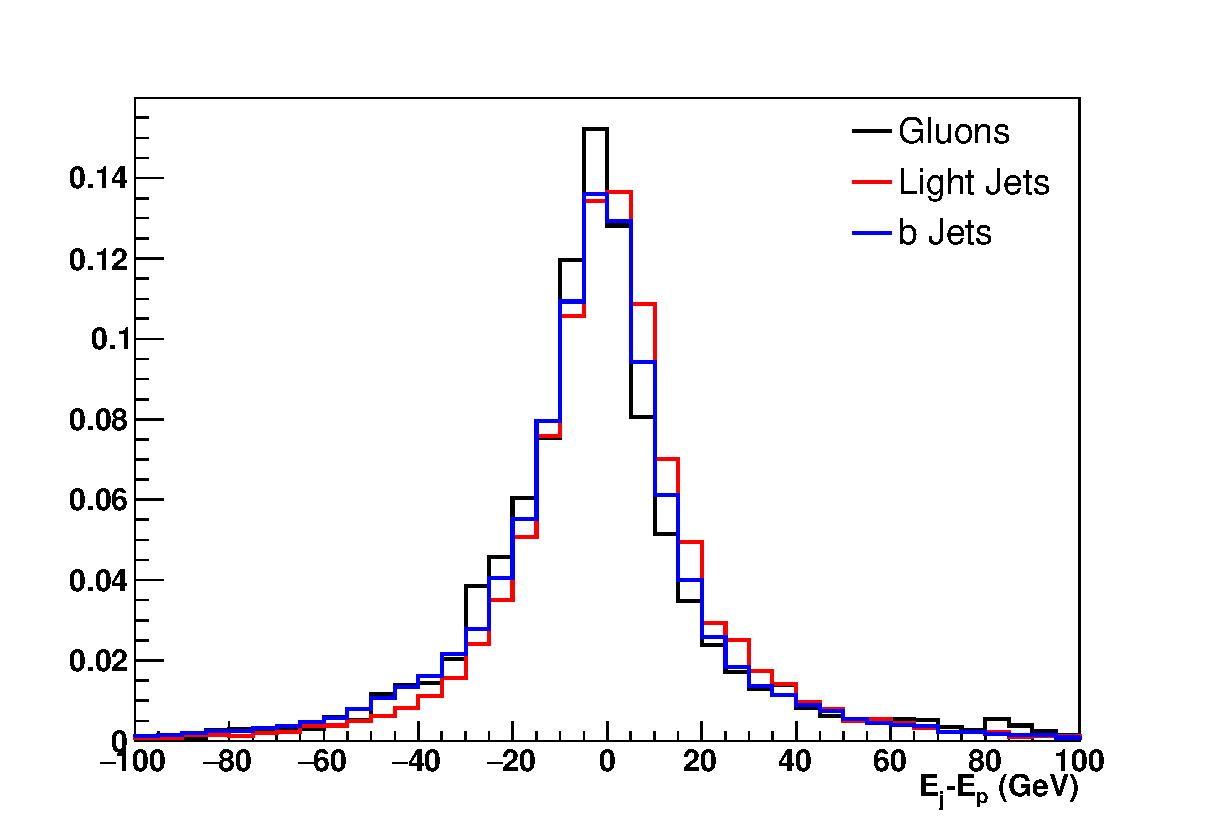
\includegraphics[width=0.95\textwidth]{\figpath/Ej-Ep.eps}
	\end{center}
\end{frame}

\begin{frame}
	\frametitle{Matrix Element Analysis}
	\framesubtitle{Using the Probability Densities}
	\vspace*{-0.24cm}

	\begin{block}{ME Combination}
		\begin{columns}[T]
			\column{0.7\textwidth}
			\begin{itemize}
				\item We still needed to combine the 15 MEs into some discriminator
				\begin{itemize}
					\item They could be combined into a likelihood as in the Matrix Element Liklihood Analysis (MELA) used by $H{\rightarrow}ZZ{\rightarrow}4\ell$ (see equation~\ref{eq:MELA})
					\item We could use an event probability discriminant (see equation~\ref{eq:epd}) as was done by CDF
					\item \textbf{We ultimately decided to use a BDT to combine the MEs}
					\begin{itemize}
						\item In escence we give a shallow network (the BDT) the ability to create a non-linear discriminant function
						\item This is possible only because the probability densities are already non-linear variables
					\end{itemize}
				\end{itemize}
			\end{itemize}
			\column{0.3\textwidth}
			\vspace*{0.7cm}
			\includegraphics[width=\textwidth]{\figpath/WDecayAngles.png}%
		\end{columns}
		\begin{aeq}{eq:MELA}
MELA=\left[1+\frac{{\color{blue}\mathcal{P}_{bkg}}\left(m_{1},m_{2},\theta_{1},\theta_{2},\Phi,\theta^{*},\Phi_{1}|m_{4\ell}\right)}{{\color{red}\mathcal{P}_{sig}}\left(m_{1},m_{2},\theta_{1},\theta_{2},\Phi,\theta^{*},\Phi_{1}|m_{4\ell}\right)}\right]^{-1}
		\end{aeq}
		\begin{aeq}{eq:epd}
EPD=\frac{\mathcal{P}_{signal1}+\mathcal{P}_{signal2}+...}{\mathcal{P}_{signal1}+\mathcal{P}_{signal2}+...+\mathcal{P}_{background1}+\mathcal{P}_{background2}+...}
		\end{aeq}
	\end{block}
\end{frame}

\begin{comment}
\begin{frame}<1>[label=frame:MEBDT_training]
	\frametitle{Matrix Element Analysis}
	\framesubtitle{MEBDT Training}
	\vspace*{-0.35cm}

	\begin{columns}[T]
		\column{0.54\textwidth}
		\vspace*{-0.25cm}
		\begin{block}{}
			\begin{itemize}
				\small
				\item \textbf{ggH (WJets)} is the dominant signal (background) in the $\geqslant2$ jets bin
				\item Training settings:
				\begin{itemize}
					\item $H{\rightarrow}WW$ as signal MC (weighted to respective fractions) and W+jets as background
					\item nTrees, maxDepth, adaBoostBeta, and nEventsMin optimized in each bin
					\item Trained on combined electron$+$muon channel
				\end{itemize}
				\item Trained in individual jet bins
				\item We investigated using the probability densities ($\mathcal{P}$) on their own, $\log{\mathcal{P}}$, $\mathcal{P}_{max}$, $\log{\mathcal{P}_{max}}$, and a combination of these
				\begin{itemize}
					\item Ultimately we decided to go with $\log{\mathcal{P}}$
				\end{itemize}
				\only<1>{\vspace*{0.80cm}}
				\only<2>{\item Signal in ({\color{blue}blue}) and W+jets background ({\color{red}red}) for the input variables to the 2 jet bin}
			\end{itemize}
		\end{block}
		\column{0.46\textwidth}
			\only<1>{
				\begin{table}[hbtp]
					\centering
					\tiny
					\begin{tabular}{| l | r |}
						\hline\hline
						Process & $\geqslant2$ Percent Yield \\
						\hline
						W$+$Jets & \cellcolor{yellow}70.25 \\
						Multi-Jet & 12.07 \\
						$t\bar{t}$ & 8.51 \\
						Z$+$Jets & 6.32 \\
						Single t   & 1.84 \\
						Diboson    & 1.01 \\
						\hline
						Total Bkg & 100.00 \\
						\hline\hline
						ggH M$_{H}=125$ & \cellcolor{yellow}47.47 \\
						qqH M$_{H}=125$ & 10.17 \\
						WH M$_{H}=125$, H${\rightarrow}b\bar{b}$ & \cellcolor{green}42.36 \\
						\hline
						Tot Sig & 100.00 \\
						\hline\hline
					\end{tabular}
					\label{tab:yields2}
				\end{table}
			}
			\only<2>{
				\centering
				\includegraphics[width=\textwidth]{\figpath/MVA/2015_07_17_TMVA_output_jets2_eq0tag_both_HToWW_WJets_allEvtProbs_0KinVar/variables_id_c1.pdf}\\
				\includegraphics[width=\textwidth]{\figpath/MVA/2015_07_17_TMVA_output_jets2_eq0tag_both_HToWW_WJets_allEvtProbs_0KinVar/variables_id_c2.pdf}\\
				\includegraphics[width=\textwidth]{\figpath/MVA/2015_07_17_TMVA_output_jets2_eq0tag_both_HToWW_WJets_allEvtProbs_0KinVar/variables_id_c3.pdf}
			}
	\end{columns}
\end{frame}
\againframe<2>{frame:MEBDT_training}

\label{sec:MEBDT_variable_selections}
\frame[shrink=0.05]{
	\frametitle{ME BDT Variable Selection}

\begin{table}[ht!] 
  \centering 
  \noindent 
  \tiny 
    \caption{The training and use settings for each binned BDT category. This table is specifically for the 0 b-tag trainings. Unless otherwise noted, all information from here on out is for the combined electron \& muon channels. The $H{\rightarrow}WW$ samples use the ggH, qqH, WH, ZH, and TTH production mechanisms.} 
    \label{tab:Table0} 
    \resizebox{\textwidth}{!}{%
    \begin{tabular}{| l | c | c | c | c | c | c | c | c |} \hline 
Setting & $\geq2$ Jets (Kin) & $\geq2$ Jets (ME) & $==2$ Jets (Kin) & $==2$ Jets (ME) & $==3$ Jets (Kin) & $==3$ Jets (ME)  & $\geq4$ Jets (Kin) & $\geq4$ Jets (ME)\\ \hline %==2 without tEvent prob & =2 jus t joey's
 
Signal Samples & $H{\rightarrow}WW$ & $H{\rightarrow}WW$ & $H{\rightarrow}WW$ & $H{\rightarrow}WW$ & $H{\rightarrow}WW$ & $H{\rightarrow}WW$ & $H{\rightarrow}WW$ & $H{\rightarrow}WW$ \\
 
Background Samples & WJets & WJets & WJets & WJets & WJets & WJets & WJets & WJets \\

B-Tags & 0 & 0 & 0 & 0 & 0 & 0 & 0 & 0 \\

Depth & 3 & 3 & 3 & 3 & 3 & 3 & 3 & 3 \\
 
\multirow{14}{*}{Variables} & $p_{T}^{Lepton}$ && ht && ht && ht & \\
& $M_{T}$ && dPhiMETJet && $p_{T}^{Lepton}$ && dPhiMETJet & \\
& $N_{Jets}$ && CosTheta\_l && CosTheta\_WH && dPhiMETLep & \\
& $M_{l{\nu}jj}$ && $p_{T}^{Lepton}$ && minDPhiLepJet&& ${\Delta}R_{lep,jet2}$ & \\
& ${\Delta}R_{lep,jet2}$ && ${\Delta}R_{lep,jet1}$ && $M_{l{\nu}jj}$ && $M_{l{\nu}jj}$ & \\
& ${\Delta}R_{lep,jet3}$ && ${\Delta}R_{lep,jet2}$ && leptonEtaCharge && ${\Delta}R_{lep,jet3}$ & \\
& ${\Delta}R_{lep,jet4}$ && dRlepjj && dEtaJetJet && leptonEtaCharge & \\
& $N_{BTags}$ && mT && CosTheta\_l && & \\
& && dPhiJetJet && CosTheta\_j && & \\
& && Ptlnujj && dPhiMETJet && & \\
& && CosTheta\_WH && ${\Delta}R_{lep,jet3}$ && & \\
& && && ${\Delta}R_{lep,jet2}$ && & \\
& && && dRlepjj && & \\
& & All tEventProbs && All tEventProbs && All tEventProbs & & All tEventProbs\\ \hline 

Bkd. Rej. at \textbf{X}$\%$ Sig. Eff. &&& 80.5(\textbf{50}) & 70.3(\textbf{50}) & 84.7(\textbf{50}) & 70.4(\textbf{50}) & 84.3(\textbf{50}) & 71.8(\textbf{50}) \\
Bkd. Rej. at \textbf{Y}$\%$ Sig. Eff. &&& 30.6(\textbf{90}) & 23.9(\textbf{90}) & 41.6(\textbf{90}) & 24.5(\textbf{90}) & 32.2(\textbf{90}) & 24.7(\textbf{90}) \\
Best Point Coord &&& (0.6591,0.6666) & (0.6061,0.6063) & (0.7093,0.6927) & (0.6141,0.6027) & (0.6582,0.7057) & (0.6254,0.6057) \\
Area Under Curve &&& 0.7231 & 0.6512 & 0.7696 & 0.6507 & 0.7448 & 0.6597 \\
FOM for ROC & & & \cellcolor{yellow}0.4769 & \cellcolor{red}0.5569 & 0.4231 & 0.5538 & 0.4511 & 0.5439 \\ \hline
K-S test: Sig. &&& 3.36e-06 & 0.000677 & 3.8e-08 & 7.07e-17 & 2.05e-21 & 3.04e-32 \\
K-S test: Bkd. &&& 0.773 & 0.333 & 0.00683 & 0.00955 & 1.59e-08 & 1.14e-16 \\ \hline
(Kin+ME) Bkd. Rej. at \textbf{X}$\%$ Sig. Eff. & \multicolumn{2}{c|}{} & \multicolumn{2}{c|}{81.2(\textbf{50})} & \multicolumn{2}{c|}{85.0(\textbf{50})} & \multicolumn{2}{c|}{85.1(\textbf{50})} \\
(Kin+ME) Bkd. Rej. at \textbf{Y}$\%$ Sig. Eff. & \multicolumn{2}{c|}{} & \multicolumn{2}{c|}{33.5(\textbf{90})} & \multicolumn{2}{c|}{41.6(\textbf{90})} & \multicolumn{2}{c|}{35.7(\textbf{90})} \\
(Kin+ME) Best Point Coord & \multicolumn{2}{c|}{} & \multicolumn{2}{c|}{(0.6727,0.6654)} & \multicolumn{2}{c|}{(0.6913,0.7087)} & \multicolumn{2}{c|}{(0.6794,0.7023)} \\
(Kin+ME) Area Under Curve & \multicolumn{2}{c|}{} & \multicolumn{2}{c|}{0.7330} & \multicolumn{2}{c|}{0.7712} & \multicolumn{2}{c|}{0.7586} \\
(Kin+ME) FOM for ROC & \multicolumn{2}{c|}{} & \multicolumn{2}{c|}{0.4681} & \multicolumn{2}{c|}{0.4244} & \multicolumn{2}{c|}{0.4375} \\ \hline
K-S test: Sig. &  \multicolumn{2}{c|}{} &  \multicolumn{2}{c|}{8.65e-06} &  \multicolumn{2}{c|}{2.56e-08} &  \multicolumn{2}{c|}{1.14e-30} \\
K-S test: Bkd. & \multicolumn{2}{c|}{} &  \multicolumn{2}{c|}{0.214} &  \multicolumn{2}{c|}{0.00111} &  \multicolumn{2}{c|}{8.71e-13} \\ \hline
    \end{tabular} }
\end{table}
}
\frame[shrink=0.05]{
	\frametitle{ME BDT Variable Selection}

\begin{table}[ht!] 
  \centering 
  \noindent 
  \tiny 
    \caption{The training and use settings for each binned BDT category. This table is specifically for the 0 b-tag trainings. Unless otherwise noted, all information from here on out is for the combined electron \& muon channels. The $H{\rightarrow}WW$ samples use the ggH, qqH, WH, ZH, and TTH production mechanisms. These are three extra cases that were tested to see if they yielded more sensitivity than the standard tEventProbs.}
    \label{tab:Table1} 
    \resizebox{\textwidth}{!}{%
    \begin{tabular}{| l | c | c | c | c | c | c | c | c | c |} \hline 
Setting & $==2$ Jets (ME) & $==2$ Jets (ME) & $==2$ Jets (ME) & $==2$ Jets & $==2$ Jets & $==3$ Jets & $==3$ Jets & $==4$ Jets & $==4$ Jets \\ \hline
Signal Samples & $H{\rightarrow}WW$ & $H{\rightarrow}WW$ & $H{\rightarrow}WW$ & $H{\rightarrow}WW$ & $H{\rightarrow}WW$ & $H{\rightarrow}WW$ & $H{\rightarrow}WW$ & $H{\rightarrow}WW$ & $H{\rightarrow}WW$ \\
Background Samples & WJets & WJets & WJets & WJets & WJets & WJets & WJets & WJets & WJets \\
B-Tags & 0 & 0 & 0 & 0 & 0 & 0 & 0 & 0 & 0 \\
Depth & 3 & 3 & 3 & 3 & 3 & 3 & 3 & 3 & 3 \\
 
\multirow{15}{*}{Variables} &&&&& ht && ht && ht \\
&&&&& dPhiMETJet && $p_{T}^{Lepton}$ && dPhiMETJet \\
&&&&& CosTheta\_l && CosTheta\_WH && dPhiMETLep \\
&&&&& $p_{T}^{Lepton}$ && minDPhiLepJet && ${\Delta}R_{lep,jet2}$ \\
&&&&& ${\Delta}R_{lep,jet1}$ && $M_{l{\nu}jj}$ && $M_{l{\nu}jj}$ \\
&&&&& ${\Delta}R_{lep,jet2}$ && leptonEtaCharge && ${\Delta}R_{lep,jet3}$ \\
&&&&& dRlepjj && dEtaJetJet && leptonEtaCharge \\
&&&&& mT && CosTheta\_l && \\
&&&&& dPhiJetJet && CosTheta\_j && \\
&&&&& Ptlnujj && dPhiMETJet && \\
&&&&& CosTheta\_WH && ${\Delta}R_{lep,jet3}$ && \\
&&&&&&& ${\Delta}R_{lep,jet2}$ && \\
& All tEventProbs & All tEventMaxProbs & All tEventProbs & All tEventProbs &  & All tEventProbs & dRlepjj & All tEventProbs &  \\
& (nonLog) & & All tEventMaxProbs & KinBDT & MEBDT & KinBDT & MEBDT & KinBDT & MEBDT \\ \hline

Bkd. Rej. at \textbf{X}$\%$ Sig. Eff. && 72.7(\textbf{50}) & 76.4(\textbf{50}) & 84.0(\textbf{50}) & 86.6(\textbf{50}) & 90.4(\textbf{50}) & 91.6(\textbf{50}) & 86.2(\textbf{50}) & 90.1(\textbf{50}) \\
Bkd. Rej. at \textbf{Y}$\%$ Sig. Eff. && 26.4(\textbf{90}) & 30.4(\textbf{90}) & 37.3(\textbf{90}) & 39.7(\textbf{90}) & 49.2(\textbf{90}) & 52.6(\textbf{90}) & 45.6(\textbf{90}) & 47.9(\textbf{90}) \\
Best Point Coord && (0.6177,0.6209) & (0.6445,0.6436) & (0.6765,0.6959) & (0.7035,0.7016) & (0.7304,0.7408) & (0.7569,0.7417) & (0.7226,0.7007) & (0.7401,0.7301) \\
Area Under Curve && 0.6691 & 0.6990 & 0.7577 & 0.7772 & 0.8179 & 0.8334 & 0.7862 & 0.8138 \\
FOM for ROC & & 0.5384 & 0.5034 & \cellcolor{cyan}0.4439 & \cellcolor{green}0.4207 & 0.3740 & 0.3547 & 0.4081 & 0.3747 \\ \hline
K-S test: Sig. & & & & 0.082 & 0.251& 0.0658 & 0.00129 & 7.32e-07 & 0.00166 \\
K-S test: Bkd. & & & & 0.942 & 0.335 & 0.00252 & 0.0191 & 7.78e-07 & 0.00197 \\ \hline
(Kin+ME) Bkd. Rej. at \textbf{X}$\%$ Sig. Eff. &&&& \multicolumn{2}{c|}{82.8(\textbf{50})} & \multicolumn{2}{c|}{89.4(\textbf{50})} & \multicolumn{2}{c|}{78.9(\textbf{50})} \\
(Kin+ME) Bkd. Rej. at \textbf{Y}$\%$ Sig. Eff. &&&& \multicolumn{2}{c|}{36.1(\textbf{90})} & \multicolumn{2}{c|}{47.8(\textbf{90})} & \multicolumn{2}{c|}{41.9(\textbf{90})} \\
(Kin+ME) Best Point Coord &&&& \multicolumn{2}{c|}{(0.6179,0.7384)} & \multicolumn{2}{c|}{(0.7249,0.7357)} & \multicolumn{2}{c|}{(0.7033,0.6776)} \\
(Kin+ME) Area Under Curve &&&& \multicolumn{2}{c|}{0.7495} & \multicolumn{2}{c|}{0.8123} & \multicolumn{2}{c|}{0.7427} \\
(Kin+ME) FOM for ROC &&&& \multicolumn{2}{c|}{0.4631} & \multicolumn{2}{c|}{0.3815} & \multicolumn{2}{c|}{0.4382} \\ \hline
K-S test: Sig. &&&&  \multicolumn{2}{c|}{0.547} &  \multicolumn{2}{c|}{0.702} &  \multicolumn{2}{c|}{0.902} \\
K-S test: Bkd. &&&&  \multicolumn{2}{c|}{3.57e-10} &  \multicolumn{2}{c|}{0.000364} &  \multicolumn{2}{c|}{1.49e-13} \\ \hline
    \end{tabular} }
\end{table}
}
\frame[shrink=0.05]{
	\frametitle{ME BDT Variable Selection}

\begin{table}[ht!] 
  \centering 
  \noindent 
  \tiny 
    \caption{The training and use settings for each binned BDT category. This table is specifically for the 1 b-tag trainings. Unless otherwise noted, all information from here on out is for the combined electron \& muon channels. The $H{\rightarrow}WW$ samples use the ggH, qqH, WH, ZH, and TTH production mechanisms.} 
    \label{tab:Table2} 
    \resizebox{\textwidth}{!}{%
    \begin{tabular}{| l | c | c | c | c | c | c | c | c |} \hline 
Setting & $\geq2$ Jets (Kin) & $\geq2$ Jets (ME) & $==2$ Jets (Kin) & $==2$ Jets (ME) & $==3$ Jets (Kin) & $==3$ Jets (ME)  & $\geq4$ Jets (Kin) & $\geq4$ Jets (ME)\\ \hline %==2 without tEvent prob & =2 jus t joey's
 
Signal Samples & $H{\rightarrow}WW$ & $H{\rightarrow}WW$ & $H{\rightarrow}WW$ & $H{\rightarrow}WW$ & $H{\rightarrow}WW$ & $H{\rightarrow}WW$ & $H{\rightarrow}WW$ & $H{\rightarrow}WW$ \\
 
Background Samples & WJets+TTbar & WJets+TTbar & WJets+TTbar & WJets+TTbar & WJets+TTbar & WJets+TTbar & WJets+TTbar & WJets+TTbar \\

B-Tags & 1 & 1 & 1 & 1 & 1 & 1 & 1 & 1 \\

Depth & 3 & 3 & 3 & 3 & 3 & 3 & 3 & 3 \\
 
\multirow{14}{*}{Variables} & $p_{T}^{Lepton}$ && ht && dPhiMETJet && dPhiMETJet & \\
& $M_{T}$ && $p_{T}^{Lepton}$ && CosTheta\_j && dRlepjj & \\
& $N_{Jets}$ && jet2dRLep && mT && ${\Delta}R_{lep,jet2}$ & \\
& $M_{l{\nu}jj}$ && jet1dRLep && CosTheta\_l && mT & \\
& ${\Delta}R_{lep,jet2}$ && CosTheta\_l && jet2Pt && sumJetEt & \\
& ${\Delta}R_{lep,jet3}$ && dEtaJetJet && ht && $p_{T}^{Lepton}$ & \\
& ${\Delta}R_{lep,jet4}$ && mT && ${\Delta}R_{lep,jet3}$ && ht & \\
& $N_{BTags}$ && dPhiMETJet && $p_{T}^{Lepton}$ && ${\Delta}R_{lep,jet3}$ & \\
& && dPhiJetJet && dRlepjj && JacobePeak & \\
& && && CosTheta\_WH && ${\Delta}R_{lep,jet4}$ & \\
& && && JacobePeak && CosTheta\_l & \\
& && && && $N_{Jets}$ & \\
& && && && CosTheta\_j & \\
& & All tEventProbs && All tEventProbs && All tEventProbs & & All tEventProbs\\ \hline 

Bkd. Rej. at \textbf{X}$\%$ Sig. Eff. &&& 76.8(\textbf{50}) & 69.4(\textbf{50}) & 84.0(\textbf{50}) & 72.6(\textbf{50}) & 87.6(\textbf{50}) & 71.5(\textbf{50}) \\
Bkd. Rej. at \textbf{Y}$\%$ Sig. Eff. &&& 26.8(\textbf{90}) & 21.7(\textbf{90}) & 37.6(\textbf{90}) & 21.1(\textbf{90}) & 36.5(\textbf{90}) & 18.3(\textbf{90}) \\
Best Point Coord &&& (0.6346,0.6437) & (0.5956,0.6047) & (0.6846,0.6911) & (0.6002,0.6343) & (0.6840,0.7291) & (0.5960,0.6170) \\
Area Under Curve &&& 0.6919 & 0.6401 & 0.7553 & 0.6572 & 0.7736 & 0.6470 \\
FOM for ROC & & & 0.5103 & 0.5655 & 0.4415 & 0.5418 & 0.4162 & 0.5567 \\ \hline
(Kin+ME) Bkd. Rej. at \textbf{X}$\%$ Sig. Eff. & \multicolumn{2}{c|}{} & \multicolumn{2}{c|}{(\textbf{50})} & \multicolumn{2}{c|}{84.8(\textbf{50})} & \multicolumn{2}{c|}{(\textbf{50})} \\
(Kin+ME) Bkd. Rej. at \textbf{Y}$\%$ Sig. Eff. & \multicolumn{2}{c|}{} & \multicolumn{2}{c|}{(\textbf{90})} & \multicolumn{2}{c|}{37.7(\textbf{90})} & \multicolumn{2}{c|}{(\textbf{90})} \\
(Kin+ME) Best Point Coord & \multicolumn{2}{c|}{} & \multicolumn{2}{c|}{} & \multicolumn{2}{c|}{(0.6975,0.6888)} & \multicolumn{2}{c|}{} \\
(Kin+ME) Area Under Curve & \multicolumn{2}{c|}{} & \multicolumn{2}{c|}{} & \multicolumn{2}{c|}{0.7608} & \multicolumn{2}{c|}{} \\
(Kin+ME) FOM for ROC & \multicolumn{2}{c|}{} & \multicolumn{2}{c|}{} & \multicolumn{2}{c|}{0.4340} & \multicolumn{2}{c|}{} \\ \hline
    \end{tabular} }
%  \end{adjustwidth} 
\end{table}
}
\end{comment}

\begin{frame}
	\frametitle{BDT Training \& Optimization}
	\framesubtitle{With Kinematic Input Variables}
	
	\includegraphics[width=0.21\textwidth]{\figpath/MVA_Variables_Examined.pdf}%
	\hspace*{0.05\textwidth}\includegraphics[width=0.21\textwidth]{\figpath/MVA_Variables_2j0B.pdf}%
	\hspace*{0.05\textwidth}\includegraphics[width=0.21\textwidth]{\figpath/MVA_Variables_3j0B.pdf}%
	\hspace*{0.05\textwidth}\includegraphics[width=0.21\textwidth]{\figpath/MVA_Variables_4j0B.pdf}%
	\begin{textblock}{0.2}(0.23,0.45){\color{red}$\Rightarrow$}\end{textblock}
	\begin{textblock}{0.2}(0.485,0.45){\color{blue}$+$}\end{textblock}
	\begin{textblock}{0.2}(0.733,0.45){\color{blue}$+$}\end{textblock}

	\includegraphics[width=0.5\textwidth]{\figpath/MVA/2015_07_17_TMVA_output_jets2_eq0tag_both_HToWW_WJets_noEvtProbs_11KinVar/variables_id_c1.pdf}%
	\includegraphics[width=0.5\textwidth]{\figpath/MVA/2015_07_17_TMVA_output_jets2_eq0tag_both_HToWW_WJets_noEvtProbs_11KinVar/variables_id_c2.pdf}%
	\begin{textblock}{0.15}(0.83,0.81){
		\includegraphics[width=\textwidth]{\figpath/MVA/2015_07_17_TMVA_output_jets2_eq0tag_both_HToWW_WJets_noEvtProbs_11KinVar/mva_BDT.pdf}%
	}\end{textblock}
\end{frame}

\begin{frame}
	\frametitle{All MVA Compared}
	\framesubtitle{Output Classifiers}

	\vspace*{-0.24cm}
	\begin{myfancyblock}
		\node[anchor=south west,inner sep=0] (image) at (0,0) {%
			\hspace*{0.3cm}\includegraphics[width=0.28\textwidth]{\figpath/MVA/2015_07_17_TMVA_output_jets2_eq0tag_both_HToWW_WJets_noEvtProbs_11KinVar/mva_BDT.pdf}%
			\includegraphics[width=0.28\textwidth]{\figpath/MVA/2015_07_17_TMVA_output_jets3_eq0tag_both_HToWW_WJets_noEvtProbs_13KinVar/mva_BDT.pdf}%
			\includegraphics[width=0.28\textwidth]{\figpath/MVA/2015_07_17_TMVA_output_jets4_eq0tag_both_HToWW_WJets_noEvtProbs_7KinVar/mva_BDT.pdf}%
		};
		\node[anchor=south west,inner sep=0] (image2) at (0,-2.60) {%
			\hspace*{0.3cm}\includegraphics[width=0.28\textwidth]{\figpath/MVA/2015_07_17_TMVA_output_jets2_eq0tag_both_HToWW_WJets_allEvtProbs_0KinVar/mva_BDT.pdf}%
			\includegraphics[width=0.28\textwidth]{\figpath/MVA/2015_07_17_TMVA_output_jets3_eq0tag_both_HToWW_WJets_allEvtProbs_0KinVar/mva_BDT.pdf}%
			\includegraphics[width=0.28\textwidth]{\figpath/MVA/2015_07_17_TMVA_output_jets4_eq0tag_both_HToWW_WJets_allEvtProbs_0KinVar/mva_BDT.pdf}%
		};
		\node[anchor=south west,inner sep=0] (image3) at (0,-5.20) {%
			\hspace*{0.3cm}\includegraphics[width=0.28\textwidth]{\figpath/MVA/2015_07_17_TMVA_output_jets2_eq0tag_both_HToWW_WJets_noEvtProbs_12KinVar/mva_BDT.pdf}%
			\includegraphics[width=0.28\textwidth]{\figpath/MVA/2015_07_17_TMVA_output_jets3_eq0tag_both_HToWW_WJets_noEvtProbs_14KinVar/mva_BDT.pdf}%
			\includegraphics[width=0.28\textwidth]{\figpath/MVA/2015_07_17_TMVA_output_jets4_eq0tag_both_HToWW_WJets_noEvtProbs_8KinVar/mva_BDT.pdf}%
		};
		\hspace*{-0.26cm}\node [draw,rectangle,text centered, rounded corners,fill=tamugray,tamugray,text=Black,rotate=90, left of = image, xshift=1.1cm, yshift=6.0cm] {Kin BDT};
		\hspace*{-0.00cm}\node [draw,rectangle,text centered, rounded corners,fill=tamugray,tamugray,text=Black,rotate=90, left of = image2, xshift=1.1cm, yshift=6.0cm] {ME BDT};
		\hspace*{-0.00cm}\node [draw,rectangle,text centered, rounded corners,fill=tamugray,tamugray,text=Black,rotate=90, left of = image3, xshift=1.1cm, yshift=6.0cm] {Kin+ME BDT};
		
	\end{myfancyblock}
	\begin{textblock}{5.0}(4.20,2.0){\color{red}{2J0B}}\end{textblock}
	\begin{textblock}{5.0}(7.70,2.0){\color{red}{3J0B}}\end{textblock}
	\begin{textblock}{5.0}(11.1,2.0){\color{red}{4J0B}}\end{textblock}

	\begin{textblock}{5.0}(4.20,4.6){\color{red}{2J0B}}\end{textblock}
	\begin{textblock}{5.0}(7.70,4.6){\color{red}{3J0B}}\end{textblock}
	\begin{textblock}{5.0}(11.1,4.6){\color{red}{4J0B}}\end{textblock}

	\begin{textblock}{5.0}(4.20,7.2){\color{red}{2J0B}}\end{textblock}
	\begin{textblock}{5.0}(7.70,7.2){\color{red}{3J0B}}\end{textblock}
	\begin{textblock}{5.0}(11.2,7.2){\color{red}{4J0B}}\end{textblock}
\end{frame}



\begin{frame}
	\frametitle{All MVA Compared}
	\framesubtitle{Receiver Operating Characteristic (ROC) Curves}

	\vspace*{-0.24cm}
	\begin{myfancyblock}
		\node[anchor=south west,inner sep=0] (image) at (0,0) {%
			\hspace*{0.3cm}\includegraphics[width=0.28\textwidth]{\figpath/MVA/2015_07_17_TMVA_output_jets2_eq0tag_both_HToWW_WJets_noEvtProbs_11KinVar/rejBvsS.pdf}%
			\includegraphics[width=0.28\textwidth]{\figpath/MVA/2015_07_17_TMVA_output_jets3_eq0tag_both_HToWW_WJets_noEvtProbs_13KinVar/rejBvsS.pdf}%
			\includegraphics[width=0.28\textwidth]{\figpath/MVA/2015_07_17_TMVA_output_jets4_eq0tag_both_HToWW_WJets_noEvtProbs_7KinVar/rejBvsS.pdf}%
		};
		\node[anchor=south west,inner sep=0] (image2) at (0,-2.60) {%
			\hspace*{0.3cm}\includegraphics[width=0.28\textwidth]{\figpath/MVA/2015_07_17_TMVA_output_jets2_eq0tag_both_HToWW_WJets_allEvtProbs_0KinVar/rejBvsS.pdf}%
			\includegraphics[width=0.28\textwidth]{\figpath/MVA/2015_07_17_TMVA_output_jets3_eq0tag_both_HToWW_WJets_allEvtProbs_0KinVar/rejBvsS.pdf}%
			\includegraphics[width=0.28\textwidth]{\figpath/MVA/2015_07_17_TMVA_output_jets4_eq0tag_both_HToWW_WJets_allEvtProbs_0KinVar/rejBvsS.pdf}%
		};
		\node[anchor=south west,inner sep=0] (image3) at (0,-5.20) {%
			\hspace*{0.3cm}\includegraphics[width=0.28\textwidth]{\figpath/MVA/2015_07_17_TMVA_output_jets2_eq0tag_both_HToWW_WJets_noEvtProbs_12KinVar/rejBvsS.pdf}%
			\includegraphics[width=0.28\textwidth]{\figpath/MVA/2015_07_17_TMVA_output_jets3_eq0tag_both_HToWW_WJets_noEvtProbs_14KinVar/rejBvsS.pdf}%
			\includegraphics[width=0.28\textwidth]{\figpath/MVA/2015_07_17_TMVA_output_jets4_eq0tag_both_HToWW_WJets_noEvtProbs_8KinVar/rejBvsS.pdf}%
		};
		\hspace*{-0.26cm}\node [draw,rectangle,text centered, rounded corners,fill=tamugray,tamugray,text=Black,rotate=90, left of = image, xshift=1.1cm, yshift=6.0cm] {Kin BDT};
		\hspace*{-0.00cm}\node [draw,rectangle,text centered, rounded corners,fill=tamugray,tamugray,text=Black,rotate=90, left of = image2, xshift=1.1cm, yshift=6.0cm] {ME BDT};
		\hspace*{-0.00cm}\node [draw,rectangle,text centered, rounded corners,fill=tamugray,tamugray,text=Black,rotate=90, left of = image3, xshift=1.1cm, yshift=6.0cm] {Kin+ME BDT};
		
	\end{myfancyblock}
	\begin{textblock}{5.0}(4.20,2.0){\color{red}{2J0B}}\end{textblock}
	\begin{textblock}{5.0}(7.70,2.0){\color{red}{3J0B}}\end{textblock}
	\begin{textblock}{5.0}(11.1,2.0){\color{red}{4J0B}}\end{textblock}

	\begin{textblock}{5.0}(4.20,5.0){\color{red}{2J0B}}\end{textblock}
	\begin{textblock}{5.0}(7.70,5.0){\color{red}{3J0B}}\end{textblock}
	\begin{textblock}{5.0}(11.1,5.0){\color{red}{4J0B}}\end{textblock}

	\begin{textblock}{5.0}(4.20,7.5){\color{red}{2J0B}}\end{textblock}
	\begin{textblock}{5.0}(7.70,7.5){\color{red}{3J0B}}\end{textblock}
	\begin{textblock}{5.0}(11.2,7.5){\color{red}{4J0B}}\end{textblock}
\end{frame}

\begin{frame}
	\frametitle{Systematic Uncertainties}
	\framesubtitle{}
	\vspace*{-0.54cm}
	\begin{columns}[T]
		\begin{column}{0.48\textwidth}
			\begin{block}{Pileup Weights}
				\begin{itemize}
					\footnotesize
					\item Uncertainty on the weights applied to correct the pileup profile
					\item Calculated by assuming a $\pm7\%$ shift in the $\sigma_{min.bias}$ of $69.4\unit{mb}$
					\item Shape changes are negligible for our input variables
				\end{itemize}
			\end{block}
			\vspace*{-0.65cm}
			\begin{table}[htbp]
			\begin{center}
				\tiny
			    \captionsetup{width=.85\textwidth}
			    \caption{Uncertainty in the expected yield}
			    \vspace*{-0.4cm}
			    \label{tab:PUWeightSys}
			    \begin{tabular}{|p{2.5cm}|c|c|c|} \hline
					Process                                    & 2 Jets    & 3 Jets  & $\geqslant$4 Jets \\\hline
					Diboson                                    & 2-5\%     & 3-6\%   & 3.5-7\%   \\
					\Wjets                                     & 3\%       & 4\%     & 4\%       \\
					\Zjets                                     & 7-8\%     & 7-8\%   & 7-8\%     \\
					\ttbar                                     & 2\%       & 2\%     & 2\%       \\
					Single \cPqt                               & 1-3\%     & 2-8\%   & 2-9\%     \\
					Multijet                                   & 0-2\%     & 0-3\%   & 0-4\%     \\\hline
					\ggH; \newline $\MH=\text{125}\gev$, \HWW           & 2-3\%     & 3\%     & 3.5\%     \\
					\qqH; \newline $\MH=\text{125}\gev$, \HWW           & 0.5-3\%   & 1-3.5\% & 2.5-4\%   \\
					\WH, \ZH, \ttH; \newline $\MH=\text{125}\gev$, \HWW & 0-3\%     & 1-3\%   & 2-3.5\%   \\\hline
					\WH, \ZH, \ttH; \newline $\MH=\text{125}\gev$, \HZZ & 0.5-3\%   & 2-4\%   & 2-4\%     \\
					\WH; $\MH=\text{125}\gev$, \newline \Hbb, \Wlv      & 0.5-3\%   & 2-4\%   & 3.5-4.5\% \\
					\ttH; $\MH=\text{125}\gev$, \Hbb           & 1.5-4.5\% & 0-2.5\% & 2-4\%     \\\hline
				\end{tabular}
			\end{center}
			\end{table}
		\end{column}
		\begin{column}{0.48\textwidth}
			\begin{block}{Jet Energy Scale}
				\begin{itemize}
					\footnotesize
					\item Jets are calibrated on CMS
					\begin{itemize}
						\footnotesize
						\item The uncertainty on the calibration results in a systematic error
						\item This affects both the rate and shape of the final distributions
					\end{itemize}
					\item Each MC sample was scaled up and down by $1\sigma$ as officially prescribed
				\end{itemize}
			\end{block}
			\vspace*{-0.65cm}
			\begin{table}[htbp]
			\begin{center}
			  	\tiny
			    \captionsetup{width=.85\textwidth}
			    \caption{Uncertainty in the expected yield}
			    \vspace*{-0.4cm}
			    \label{tab:JESWeightSys}
			    \begin{tabular}{|p{2.5cm}|c|c|c|} \hline
					Process                                    & 2 Jets  & 3 Jets  & $\geqslant$4 Jets \\\hline
					Diboson                                    & 1-2\%   & 2\%     & 2\%     \\
					\Zjets                                     & 0-5.5\% & <1\%    & <1\%    \\
					\ttbar                                     & 8-19\%  & 4-7\%   & 2-4\%   \\
					Single \cPqt                               & 2-0\%   & <1\%    & <1\%    \\\hline
					\ggH; \newline $\MH=\text{125}\gev$, \HWW           & 0-5\%   & 0-2\%   & 0-3\%   \\
					\qqH; \newline $\MH=\text{125}\gev$, \HWW           & <1\%    & 4\%     & 7\%     \\
					\WH, \ZH, \ttH; \newline $\MH=\text{125}\gev$, \HWW & 2-3\%   & 0-5\%   & 5-8\%   \\\hline
					\WH, \ZH, \ttH; \newline $\MH=\text{125}\gev$, \HZZ & 1.5\%   & 0-6\%   & 4-5\%   \\
					\WH; $\MH=\text{125}\gev$, \newline \Hbb, \Wlv      & 8-9\%   & 1-10\%  & 2-13\%  \\
					\ttH; $\MH=\text{125}\gev$, \Hbb           & 4-17\%  & 11-24\% & 18-21\% \\\hline
				\end{tabular}
			\end{center}
			\end{table}
		\end{column}
	\end{columns}
\end{frame}